\chapter{LAB 02: Running User Programs and System Calls}

\section{The Need for System Calls}
The primary objective of an operating system is to safely and efficiently execute user-level programs. In the base distribution of OS161, user programs cannot execute correctly because the boundary separating user-space from kernel-space is incomplete. 

Specifically, when a user program attempts to perform input/output operations or attempts to terminate gracefully, the system crashes. For example, executing the palindrome test program from the OS161 menu (\texttt{p testbin/palin}) results in a kernel panic indicating "Unknown syscall 55" followed by "Unknown syscall 3". 

These failures occur because the MIPS emulator traps into the kernel upon encountering a \texttt{syscall} instruction, but the kernel lacks the implementation to handle these specific requests. Syscall 55 corresponds to \texttt{SYS\_write}, which is invoked by the C standard library's \texttt{printf} function to output text. Syscall 3 corresponds to \texttt{SYS\_\_exit}, which is implicitly called at the termination of the \texttt{main()} function to instruct the operating system to clean up the process's resources. Without these, user programs cannot communicate with the console or terminate without bringing down the entire system.

\section{The Trap Mechanism: Trapframe vs Switchframe}
To understand how system calls are intercepted, one must understand how the kernel handles execution state. In OS161, there are two primary structures used to save the CPU registers, but they serve completely different purposes and are triggered by different events: the \textbf{Trapframe} and the \textbf{Switchframe}.

\subsection{The Trapframe}

\begin{tcolorbox}[colback=red!5!white, colframe=red!75!black, title=\textbf{! EXAM FOCUS: IMPLEMENTATION REQUIRED}]
\textbf{Function:} \texttt{thread\_fork(const char *name, struct proc *proc, ...)} \\
\textbf{Exam Task:} \textit{Line-by-Line Analysis \& Trapframe} \\
You must explain what the \texttt{entrypoint} is, clarify that the allocated \texttt{STACK\_SIZE} is for the kernel stack (not user stack), and determine whether \texttt{thread\_make\_runnable} executes the thread immediately (No, it just queues it). Also, be able to distinguish whether a \texttt{trapframe} or \texttt{switchframe} is used.
\end{tcolorbox}

A \textbf{trapframe} is automatically created when the hardware transitions from user mode to kernel mode due to an exception (such as a system call, an interrupt, or a fault like accessing invalid memory). 
When a user program executes the MIPS \texttt{syscall} instruction, the hardware forces a trap. The low-level assembly handler (\texttt{mips\_trap}) immediately pushes a trapframe onto the \textbf{kernel stack} of the currently running thread. This trapframe contains the exact state of all user-space registers at the exact moment the trap occurred. This is vital because the kernel will now use the CPU, overwriting registers; the trapframe ensures that when the system call finishes, the kernel can perfectly restore the user program's state so it can resume execution seamlessly.

\begin{figure}[h]
    \centering
    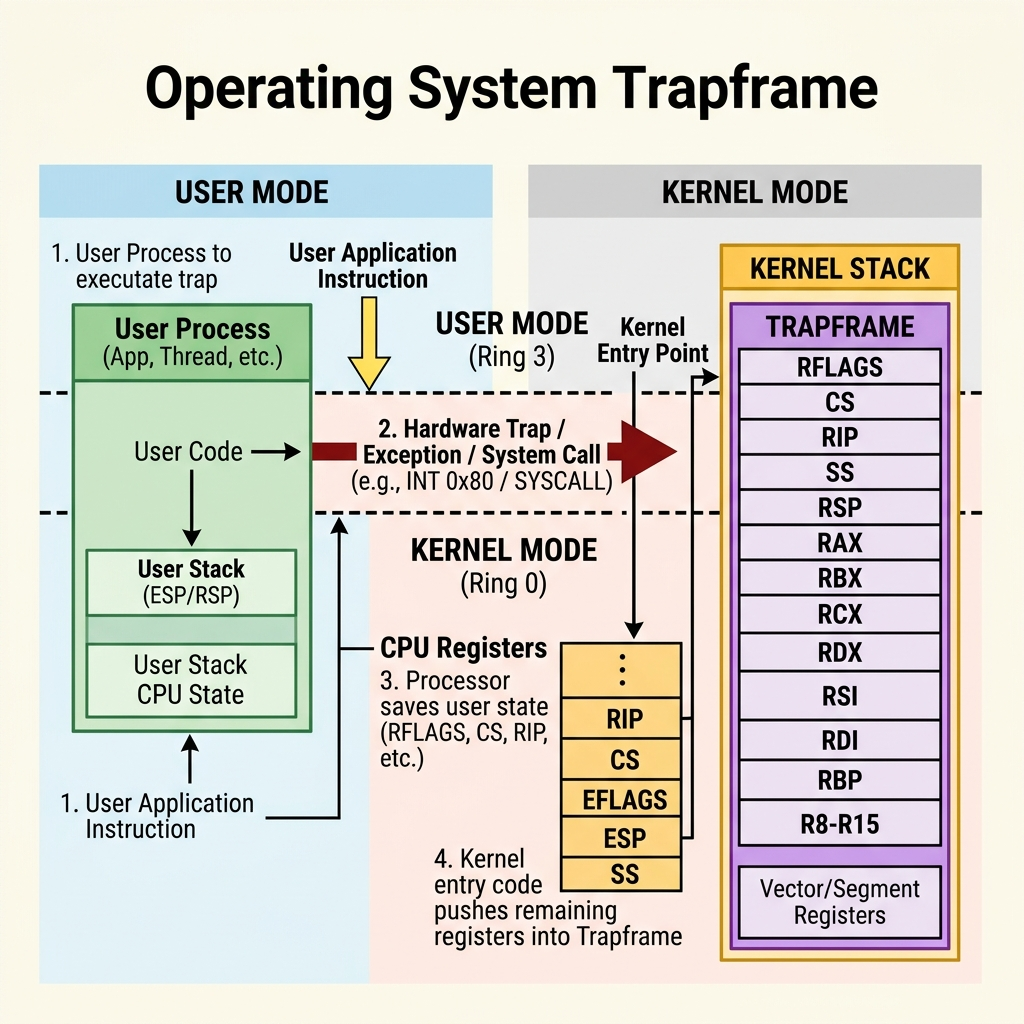
\includegraphics[width=0.8\textwidth]{images/trapframe_exception.png}
    \caption{Exception Handling and Trapframe Creation}
    \label{fig:trapframe}
\end{figure}

\subsection{The Switchframe}
A \textbf{switchframe}, on the other hand, is a purely software-driven construct. It is used exclusively during a \textbf{context switch} tra two kernel threads (i.e., when \texttt{thread\_switch} is called). 
Unlike a trapframe which saves user state, a switchframe saves the \textit{kernel} execution state (specifically, the callee-saved registers required by the C calling convention). When a thread voluntarily yields the CPU (or is preempted), it pushes a switchframe onto its \textbf{kernel stack}. When the scheduler later selects this thread to run again, it pops the switchframe off the stack, restoring the kernel registers and resuming execution exactly where it left off inside the kernel.

In summary, a trapframe handles the user-to-kernel boundary (hardware-driven), while a switchframe handles the kernel-to-kernel thread switching boundary (software-driven). Both are allocati on the \textbf{kernel stack} of the respective thread.

\section{Process Execution: From Menu to User Mode}
Understanding how a user program is actually launched requires tracing the execution path from the kernel menu. When the command \texttt{p testbin/palin} is issued, the \texttt{cmd\_prog} function is invoked. This function acts as a wrapper, calling \texttt{common\_prog}, which sets up the new process environment.

The execution trace follows this specific flow:

\begin{verbatim}
[Kernel Menu Thread]
 |___ cmd_prog("p testbin/palin")
      |___ common_prog()
           |
           |--- 1. proc_create_runprogram()
           |      (Allocates raw process data structure)
           |
           |--- 2. thread_fork("cmd_progthread")
           |      (Spawns a new kernel thread attached to the process)
           |
[New Kernel Thread Execution]
 |___ cmd_progthread()
      |___ runprogram("testbin/palin")
           |
           |--- 3. vfs_open()
           |      (Opens the executable file from disk)
           |
           |--- 4. as_create() & load_elf()
           |      (Parses ELF headers, allocates physical memory frames,
           |       and loads code/data segments into RAM)
           |
           |--- 5. as_define_stack()
           |      (Allocates the user stack area)
           |
           |___ 6. enter_new_process()
                  (Forges a Trapframe, drops privileges, and executes 
                   an assembly jump into User Mode!)
\end{verbatim}

\subsection{Deep Dive: \texttt{load\_elf} and Executable Loading}
When \texttt{runprogram} launches a user program, it opens the binary file via \texttt{vfs\_open}. The binary is formatted as an \textbf{ELF (Executable and Linkable Format)} file. The \texttt{load\_elf} function is responsible for parsing this file, configuring the virtual address space, and loading its contents into physical RAM.

The ELF file is composed of various segments. The primary ones include:
\begin{itemize}
    \item \textbf{Code Segment}: Contains \texttt{.text} (the actual executable instructions) and \texttt{.rodata} (read-only global data).
    \item \textbf{Data Segment}: Contains \texttt{.data} (initialized global data), \texttt{.bss} (uninitialized global data), and \texttt{.sbss} (small uninitialized global data).
\end{itemize}

Understanding the internal structure of \texttt{load\_elf} is critical for exam preparation, as it orchestrates the memory setup. Here is the high-level implementation structure:

\begin{lstlisting}[language=C]
int load_elf(struct vnode *v, vaddr_t *entrypoint) {
    Elf_Ehdr eh;   // ELF Header
    Elf_Phdr ph;   // Program Header
    struct addrspace *as = proc_getas();

    /* 1. Read and verify ELF Header magic number */
    read_elf_header(v, &eh);

    /* 2. Define Logical Regions */
    for (int i = 0; i < eh.e_phnum; i++) {
        read_program_header(v, &ph);
        if (ph.p_type == PT_LOAD) {
            /* Sets logical addresses and sizes for Code/Data segments */
            as_define_region(as, ph.p_vaddr, ph.p_memsz, ...);
        }
    }

    /* 3. Allocate Physical Memory */
    as_prepare_load(as);

    /* 4. Load Segments from Disk to RAM */
    for (int i = 0; i < eh.e_phnum; i++) {
        read_program_header(v, &ph);
        if (ph.p_type == PT_LOAD) {
            /* Reads the actual Code or Data segment from the ELF file */
            load_segment(as, v, ph.p_offset, ph.p_vaddr, ...);
        }
    }

    /* 5. Finalize the Address Space */
    as_complete_load(as);

    *entrypoint = eh.e_entry;
    return 0;
}
\end{lstlisting}

\subsubsection{The Core Memory Loading Functions}
As seen in the skeleton above, \texttt{load\_elf} delegates its heavy lifting to four critical functions. Understanding their exact responsibilities and execution order gives logical sense to the process creation chain (and is a frequent exam topic, e.g., Exam 2024-07-11 Q4.B):

\begin{enumerate}
    \item \textbf{\texttt{as\_define\_region}}: Called in the initial loop for each Program Header, this function is responsible for \textbf{setting the logical addresses and dimensions} of the code and data segments. It registers the starting virtual address (\texttt{VStart}) and the region's size inside the \texttt{addrspace} structure, but it does \textit{not} allocate physical RAM yet.
    \item \textbf{\texttt{as\_prepare\_load}}: After all logical regions are defined, this function is called to \textbf{allocate the address space in physical memory}. It officially secures the physical RAM frames necessary to host the process. In \texttt{dumbvm}, this is where \texttt{getppages()} is triggered under the hood.
    \item \textbf{\texttt{load\_segment} (For Code)}: This function is responsible for the \textbf{physical transfer of bytes} from the ELF file on disk (via the \texttt{vnode}) directly into the newly allocated RAM. 
    \item \textbf{\texttt{load\_segment} (For Data)}: \textit{Attention:} \texttt{load\_segment} is a highly generic function. The ELF loader makes absolutely no distinction between code and data segments at load time. It utilizes the exact same \texttt{load\_segment} function to transfer \textit{any} loadable segment from the disk into memory.
    \item \textbf{\texttt{as\_complete\_load}}: This function is called at the very end of the entire loading process. Its main purpose is to finalize the setup, which usually involves configuring memory permissions (such as enforcing read-only protections on the newly loaded code segment).
\end{enumerate}
Finally, \texttt{load\_elf} returns the \texttt{entrypoint} address, which \texttt{enter\_new\_process} will push into the \texttt{epc} register of the Trapframe so the CPU knows where to start executing in User Mode.

\section{The Syscall Dispatcher}
When the user code eventually needs kernel assistance—such as printing a character—it executes the MIPS \texttt{syscall} instruction. This hardware trap pushes the trapframe and routes execution to the \texttt{syscall(struct trapframe *tf)} dispatcher function located in \texttt{kern/arch/mips/syscall/syscall.c}. 

In the MIPS calling convention, the first four arguments to a function or system call are stored in registers \texttt{a0, a1, a2, a3}, and the system call identifier (the \texttt{callno}) itself is stored in register \texttt{v0}. 

The dispatcher uses a \texttt{switch} statement based on \texttt{tf->tf\_v0} to route the call to the appropriate handler (e.g., \texttt{sys\_write}).

\begin{lstlisting}[language=C]
// Modifications inside syscall(struct trapframe *tf) in kern/arch/mips/syscall/syscall.c
#if OPT_SYSCALLS
    case SYS_write:
        retval = sys_write((int)tf->tf_a0,
                (userptr_t)tf->tf_a1,
                (size_t)tf->tf_a2);
        if (retval < 0) err = ENOSYS; 
        else err = 0;
        break;
        
    case SYS__exit:
        sys__exit((int)tf->tf_a0);
        /* sys__exit does not return; the thread is destroyed inside */
        panic("sys__exit returned!\n");
        break;
#endif
\end{lstlisting}

At the end of the \texttt{syscall} function, the trapframe is modified to reflect the result back to the user process: if successful, \texttt{tf->tf\_v0} holds the return value and \texttt{tf->tf\_a3} is cleared to 0. If an error occurred, \texttt{tf->tf\_v0} holds the error code and \texttt{tf->tf\_a3} is set to 1. Crucially, the program counter \texttt{tf->tf\_epc} is incremented by 4 bytes (one instruction length) to ensure the CPU does not continuously re-execute the \texttt{syscall} instruction upon returning to user mode.

\section{Implementing File I/O and Memory Protection}
The implementations for the file-related system calls are placed in a new file, \texttt{kern/syscall/file\_syscalls.c}. The objective is to map standard output (file descriptor 1) to the console.

A naive implementation of \texttt{sys\_write} might simply cast the user's buffer pointer to a C string and iterate over it, calling \texttt{putch()} for every character. However, this is a \textbf{catastrophic security vulnerability}.

\subsection{Visualizing Logical Memory and The Danger of \texttt{kseg0}}
In the MIPS architecture, the 32-bit logical memory space (4GB) is strictly partitioned by the hardware:

\begin{verbatim}
0xFFFFFFFF +------------------------+
           | kseg2 (Kernel Mapped)  | (1 GB)
0xC0000000 +------------------------+
           | kseg1 (Kernel Uncached)| (512 MB)
0xA0000000 +------------------------+
           | kseg0 (Kernel Cached)  | (512 MB) <-- Direct map to Physical RAM
0x80000000 +========================+ 
           |                        |
           |                        |
           | kuseg (User Space)     | (2 GB) <-- User programs live HERE
           |                        |
           |                        |
0x00000000 +------------------------+
\end{verbatim}

The hardware Memory Management Unit (TLB) strictly enforces this boundary: if a user program executing in user mode attempts to read or write to an address $\geq$ \texttt{0x80000000} (like \texttt{kseg0}), the hardware immediately generates a Segmentation Fault and kills the process.

However, when a user program executes the \texttt{syscall} instruction, the CPU switches into \textbf{kernel mode} to handle the request. If a malicious user program passes a pointer pointing to \texttt{kseg0} into \texttt{sys\_write}, and the kernel blindly dereferences it (e.g., \texttt{char c = *user\_ptr}), the hardware will \textbf{allow} the access because the CPU is currently executing with kernel privileges! The malicious user program has successfully tricked the kernel into reading or overwriting its own internal memory, compromising the entire operating system.

\subsection{The Solution: \texttt{copyin} and \texttt{copyout}}

\begin{tcolorbox}[colback=red!5!white, colframe=red!75!black, title=\textbf{! EXAM FOCUS: IMPLEMENTATION REQUIRED}]
\textbf{Function:} \texttt{sys\_read(int fd, userptr\_t buf, int size)} \\
\textbf{Exam Task:} \textit{Bug Detection \& Fix} \\
In past exams, a flawed implementation of \texttt{sys\_read} is provided using \texttt{kgets} directly on \texttt{buf}. You must identify the security flaw (kernel memory overwrite via malicious pointer) and propose a fix: allocate a temporary kernel buffer, read data into it, and safely transfer to user space using \texttt{copyout()}.
\end{tcolorbox}

To prevent this, the kernel must never trust user-provided pointers. It must rigorously validate that the pointer resides entirely within the safe bounds of \texttt{kuseg}. OS161 provides specialized functions for this. Note how they utilize a special \texttt{copyfail} fault handler to safely trap bad memory accesses without causing a kernel panic:

\begin{lstlisting}[language=C]
/*
 * Copy a block of memory of length LEN from user-level address USERSRC
 * to kernel address DEST. We can use memcpy because it's protected by
 * the tm_badfaultfunc/copyfail logic.
 */
int copyin(const_userptr_t usersrc, void *dest, size_t len)
{
	int result;
	size_t stoplen;

	result = copycheck(usersrc, len, &stoplen);
	if (result) return result;
	
	if (stoplen != len) return EFAULT;

	curthread->t_machdep.tm_badfaultfunc = copyfail;

	result = setjmp(curthread->t_machdep.tm_copyjmp);
	if (result) {
		curthread->t_machdep.tm_badfaultfunc = NULL;
		return EFAULT;
	}

	memcpy(dest, (const void *)usersrc, len);

	curthread->t_machdep.tm_badfaultfunc = NULL;
	return 0;
}
\end{lstlisting}

And similarly for sending data back to the user:
\begin{lstlisting}[language=C]
/*
 * Copy a block of memory of length LEN from kernel address SRC to
 * user-level address USERDEST. We can use memcpy because it's
 * protected by the tm_badfaultfunc/copyfail logic.
 */
int copyout(const void *src, userptr_t userdest, size_t len)
{
    /* Identical fault protection as copyin, using memcpy to userdest */
    // ...
	memcpy((void *)userdest, src, len);
    // ...
	return 0;
}
\end{lstlisting}

\begin{tcolorbox}[colback=blue!5!white,colframe=blue!75!black,title=Exam Insight: System File Table vs User File Table (e.g. Q5 2022-06-20)]
\textbf{The Dual-Table Architecture:} When implementing file system calls in OS161, you typically manage two distinct tables:
\begin{itemize}
    \item \textbf{\texttt{systemFileTable} (Global):} Tracks all open files across the \textit{entire} operating system. It holds the \texttt{vnode} (the physical file on disk), the global read/write \texttt{offset}, and a \texttt{refcount} tracking how many processes are currently sharing this file.
    \item \textbf{\texttt{fileTable} (Per-Process):} An array inside \texttt{struct proc}. The index of this array is what user-space knows as the \textbf{File Descriptor (FD)}. Each entry simply contains a pointer to a specific row in the global \texttt{systemFileTable}.
\end{itemize}
\textbf{Why this separation?} It ensures isolation and security. A process only knows about small integers (FDs like 0, 1, 2) and cannot arbitrarily access files opened by other processes. The kernel uses the FD as an index into the process's \texttt{fileTable} to securely resolve the pointer to the global \texttt{systemFileTable}.

\textbf{Shared Entries and \texttt{lseek}:}
Suppose \texttt{P1->fileTable[5]} and \texttt{P2->fileTable[8]} both point to the \textit{exact same} \texttt{\&systemFileTable[20]}.
\begin{itemize}
    \item \textbf{File Descriptors:} P1 is accessing the file via FD 5. P2 is accessing the file via FD 8.
    \item \textbf{Interactivity:} Are their reads independent? \textbf{NO!} Because both FDs point to the exact same underlying \texttt{systemFileTable} entry, they inherently share the \textit{same} \texttt{offset} variable. 
    \item \textbf{The effect of \texttt{lseek}:} If P1 executes \texttt{lseek(5, ...)}, it modifies the shared \texttt{offset} in \texttt{systemFileTable[20]}. Therefore, P1's \texttt{lseek} will \textbf{SEMPRE} (always) affect P2's next \texttt{read()}, regardless of whether the seek was \texttt{SEEK\_SET}, \texttt{SEEK\_CUR}, or \texttt{SEEK\_END}.
\end{itemize}
\end{tcolorbox}

\section{Process Termination Constraints: The Suicide Paradox}
Process termination is handled in \texttt{kern/syscall/proc\_syscalls.c}. When a program calls \texttt{exit}, its resources must be reclaimed. 

A logical first thought would be to simply call \texttt{as\_destroy()} to free the memory, and then \texttt{proc\_destroy()} to destroy the process structure. However, a thread cannot call \texttt{proc\_destroy(curproc)} directly from within \texttt{sys\_exit}. This is known as the "suicide paradox."

Examine the implementation of \texttt{proc\_destroy()}:
\begin{lstlisting}[language=C]
void proc_destroy(struct proc *proc)
{
	KASSERT(proc != NULL);
	KASSERT(proc != kproc);

	/* VFS fields */
	if (proc->p_cwd) {
		VOP_DECREF(proc->p_cwd);
		proc->p_cwd = NULL;
	}

	/* VM fields */
	if (proc->p_addrspace) {
        /* Safely detach and destroy the address space */
		struct addrspace *as;
		if (proc == curproc) {
			as = proc_setas(NULL);
			as_deactivate();
		} else {
			as = proc->p_addrspace;
			proc->p_addrspace = NULL;
		}
		as_destroy(as);
	}

    /* THE PARADOX: Asserting the thread array is empty */
	KASSERT(proc->p_numthreads == 0);
	spinlock_cleanup(&proc->p_lock);

	proc_end_waitpid(proc);
	kfree(proc->p_name);
	kfree(proc);
}
\end{lstlisting}

To fully grasp why \texttt{proc\_destroy()} is so tricky to call correctly, we must consider what happens when a program terminates via \texttt{sys\_exit()} under three different scenarios:

\subsubsection*{Scenario A: The Memory Leak}
If your \texttt{sys\_exit()} implementation simply calls \texttt{thread\_exit()} without dealing with the process structure, the thread successfully dies. However, nobody ever called \texttt{proc\_destroy()}. The physical memory allocated to the user program (its Address Space) and the \texttt{struct proc} remain allocated in RAM forever. \textbf{This causes a severe memory leak.}

\subsubsection*{Scenario B: The Kernel Panic}
To fix the memory leak, your first instinct is to call \texttt{proc\_destroy(curproc)} right before calling \texttt{thread\_exit()}. 
However, \texttt{proc\_destroy()} contains this exact assertion: \texttt{KASSERT(proc->p\_numthreads == 0);}.
The kernel explicitly asserts that a process \textbf{must have zero active threads} before it can be safely destroyed. Since the thread executing \texttt{sys\_exit()} is still alive inside the process, \texttt{p\_numthreads} is 1. The assertion fails, resulting in an immediate \textbf{Kernel Panic}.

Even if we removed that assertion, it would still be catastrophic: the \texttt{proc\_destroy} function would deallocate the process data structures, including the thread array and potentially triggering the cleanup of the very kernel stack the thread is currently executing on. The thread would find itself executing code on memory that has just been deallocated.

\subsubsection*{Scenario C: The Correct Approach (The Zombie State)}

\begin{tcolorbox}[colback=red!5!white, colframe=red!75!black, title=\textbf{! EXAM FOCUS: IMPLEMENTATION REQUIRED}]
\textbf{Function:} \texttt{my\_sys\_exit(int status)} \\
\textbf{Exam Task:} \textit{Bug Detection \& Context Switch Analysis} \\
Exams present a buggy \texttt{my\_sys\_exit} calling \texttt{thread\_exit(curthread)} followed by \texttt{proc\_destroy(curproc)}. You must identify that calling \texttt{proc\_destroy} on the currently running process is fatal: it destroys the address space and stack the thread is actively using, causing a Kernel Panic. The thread must mark itself as a zombie and let the parent call \texttt{proc\_destroy} via \texttt{waitpid}.
\end{tcolorbox}

To safely destroy the process without panicking the kernel, and without losing the exit code before \texttt{waitpid()} is called, we split the cleanup duties:
\begin{enumerate}
    \item \textbf{The Child:} In \texttt{sys\_exit()}, the child destroys its heavy memory (the address space), detaches its thread from the process via \texttt{proc\_remthread(curthread)} (which drops \texttt{p\_numthreads} to 0), saves its exit code, marks itself as a \textbf{ZOMBIE}, and calls \texttt{thread\_exit()}. The empty \texttt{struct proc} shell remains.
    \item \textbf{The Parent:} Later, the parent calls \texttt{sys\_waitpid()}, reads the exit code, and \textit{finally} calls \texttt{proc\_destroy()} on the zombie child. Since the child's threads are gone (\texttt{p\_numthreads == 0}), the assertion passes and the memory is safely freed!
\end{enumerate}

\begin{figure}[htbp]
\centering
\begin{tikzpicture}[node distance=1.2cm and 1cm, scale=0.8, every node/.style={transform shape}]
\tikzstyle{action} = [rectangle, rounded corners, minimum width=3.5cm, minimum height=1cm,text centered, draw=cyan!80!black, fill=cyan!10]
\tikzstyle{bad} = [rectangle, minimum width=3.5cm, minimum height=1.2cm, text centered, draw=red!80!black, fill=red!10, text width=4cm]
\tikzstyle{good} = [rectangle, minimum width=3.5cm, minimum height=1.2cm, text centered, draw=green!60!black, fill=green!10, text width=4cm]
\tikzstyle{decision} = [diamond, aspect=2, minimum width=3.5cm, minimum height=1cm, text centered, draw=purple, fill=purple!10, text width=2.5cm]
\tikzstyle{arrow} = [thick,->,>=stealth]

\node (start) [action] {User calls \texttt{exit()}};
\node (sysexit) [action, below=0.6cm of start] {Kernel: \texttt{sys\_exit()}};

% Scenario A: Memory Leak
\node (scenA) [action, below left=1.2cm and 0.5cm of sysexit] {Call \texttt{thread\_exit()}};
\node (leak) [bad, below=0.8cm of scenA] {Thread dies.\\\texttt{struct proc} remains.\\\textbf{MEMORY LEAK!}};

% Scenario B: Kernel Panic
\node (scenB) [action, below=1.2cm of sysexit] {Call \texttt{proc\_destroy()}};
\node (assert) [decision, below=0.8cm of scenB] {\texttt{numthreads==0}?};
\node (panic) [bad, below=0.8cm of assert] {False! Thread is alive.\\\textbf{KERNEL PANIC!}};

% Scenario C: Zombie
\node (scenC1) [action, below right=1.2cm and 0.5cm of sysexit] {Detach thread (\texttt{proc\_remthread})};
\node (scenC2) [action, below=0.5cm of scenC1] {Mark ZOMBIE \& Save Status};
\node (scenC3) [action, below=0.5cm of scenC2] {Call \texttt{thread\_exit()}};
\node (scenC4) [action, below=0.5cm of scenC3] {Parent calls \texttt{waitpid()}};
\node (scenC5) [action, below=0.5cm of scenC4] {Parent calls \texttt{proc\_destroy()}};
\node (success) [good, below=0.5cm of scenC5] {Thread is gone.\\\textbf{SUCCESS! Memory Freed.}};

\draw [arrow] (start) -- (sysexit);
\draw [arrow] (sysexit) -- node[anchor=south east, font=\small\bfseries] {Scenario A} (scenA);
\draw [arrow] (scenA) -- (leak);

\draw [arrow] (sysexit) -- node[anchor=west, font=\small\bfseries] {Scenario B} (scenB);
\draw [arrow] (scenB) -- (assert);
\draw [arrow] (assert) -- node[anchor=west, font=\small\bfseries] {No} (panic);

\draw [arrow] (sysexit) -- node[anchor=south west, font=\small\bfseries] {Scenario C} (scenC1);
\draw [arrow] (scenC1) -- (scenC2);
\draw [arrow] (scenC2) -- (scenC3);
\draw [arrow] (scenC3) -- (scenC4);
\draw [arrow] (scenC4) -- (scenC5);
\draw [arrow] (scenC5) -- (success);
\end{tikzpicture}
\caption{Visualization of the three process termination scenarios: Memory Leak, Kernel Panic, and the Correct Zombie Implementation.}
\end{figure}

\section{Memory Management: Upgrading DumbVM}
OS161's baseline virtual memory manager, \texttt{dumbvm.c}, is exceptionally primitive. Physical memory is allocated by a function named \texttt{ram\_stealmem}.

\subsection{The Flaw of \texttt{ram\_stealmem}}

\begin{tcolorbox}[colback=red!5!white, colframe=red!75!black, title=\textbf{! EXAM FOCUS: IMPLEMENTATION REQUIRED}]
\textbf{Function:} \texttt{ram\_stealmem(unsigned long npages)} \\
\textbf{Exam Task:} \textit{Line-by-Line Analysis} \\
Exams ask whether \texttt{ram\_stealmem} allocates memory sequentially (Yes) and if it interleaves user/kernel pages (No, it's naive). You may also be asked if a free-list could replace the DumbVM bitmap (Yes, for tracking disjoint free pages).
\end{tcolorbox}

Take a close look at the original implementation of \texttt{ram\_stealmem}, which is called heavily during boot and user program execution:
\begin{lstlisting}[language=C]
paddr_t ram_stealmem(unsigned long npages)
{
	size_t size;
	paddr_t paddr;

	size = npages * PAGE_SIZE;

	if (firstpaddr + size > lastpaddr) {
		return 0; // Out of memory
	}

	paddr = firstpaddr;
	firstpaddr += size;

	return paddr;
}
\end{lstlisting}

\texttt{ram\_stealmem} allocates memory incrementally. It simply takes the first available physical address (\texttt{firstpaddr}), advances the pointer upward by the requested size, and returns the old pointer. 

The fatal flaw of \texttt{ram\_stealmem} is that it implements \textit{allocation without free}. There is no data structure recording which blocks were allocated, nor any mechanism to move \texttt{firstpaddr} backward if a middle block is freed. Consequently, repeated execution of user programs inevitably exhausts all physical RAM. Furthermore, because user memory and kernel memory are allocated from the exact same advancing pointer, the physical partitions of the kernel and user processes are permanently interlaced.

To resolve the memory leak, \texttt{dumbvm.c} must be upgraded to track the allocation state of individual physical memory frames. There are two primary architectural solutions.

\subsection{Proposed Solution 1: Bitmap Allocation}
This solution introduces two parallel arrays initialized dynamically during \texttt{vm\_bootstrap} based on the size of the physical RAM: 

\begin{lstlisting}[language=C]
static unsigned char *freeRamFrames = NULL; // 0 = free, 1 = occupied
static unsigned long *allocSize = NULL;     // Number of contiguous frames
static int nRamFrames = 0;                  // Total frames in system
\end{lstlisting}

1. A \textbf{bitmap array} (\texttt{freeRamFrames}), where a boolean value indicates whether a specific frame is free or occupied.
2. An \textbf{allocSize array}, which records the number of contiguous pages allocated starting at a given frame index. This is strictly required because when \texttt{free\_kpages} is called with a single starting address, the kernel must know exactly how many subsequent frames belong to that specific allocation to free them correctly.

\textbf{PROs:}
*   **Simplicity:** Very easy to reason about and implement.
*   **Rapid Freeing:** Deallocation is $O(1)$ relative to the number of blocks; you just iterate \texttt{allocSize} times and flip the bitmap to 0.

\textbf{CONs:}
*   **Memory Overhead:** The arrays themselves consume physical RAM permanently (one byte plus one unsigned long for every frame in the system).
*   **Slow Allocation:** Finding a free block of size N requires a linear $O(N)$ scan of the bitmap looking for a contiguous streak of zeros.

\subsection{Proposed Solution 2: Free-List Allocation}
While a bitmap is simple, an alternative implementation uses a \textbf{Free-List}—a linked list tracking only the available free intervals. The list nodes store a physical start address and a size.

\textbf{PROs:}
*   **No Static Overhead:** The list nodes can be embedded directly within the unused physical frames themselves, consuming exactly zero bytes of active system memory.
*   **Extremely Fast Best-Fit:** If the list is ordered by size, finding the tightest-fitting memory block is incredibly fast (just traverse the list until you hit the first block large enough).

\textbf{CONs:}
*   **Complex Pointer Manipulation:** Linking nodes across physical memory requires careful translation between physical and kernel virtual addresses.
*   **Slow Merging:** To combat external fragmentation, when a block is freed, the allocator must search the list to see if the adjacent physical blocks are also free to merge them. If the list is ordered by size, finding physically adjacent blocks requires an $O(N)$ search.

\subsection{Address Space Duplication (\texttt{as\_copy})}

\begin{tcolorbox}[colback=red!5!white, colframe=red!75!black, title=\textbf{! EXAM FOCUS: IMPLEMENTATION REQUIRED}]
\textbf{Function:} \texttt{as\_copy(struct addrspace *old, struct addrspace **ret)} \\
\textbf{Exam Task:} \textit{Line-by-Line Analysis \& CoW Limitations} \\
The exam asks you to analyze the deep-copy implementation of \texttt{as\_copy}. You must explain why \texttt{PADDR\_TO\_KVADDR} is strictly required (mapping physical frames into the kernel's virtual segment to perform the memmove), and observe that this deep-copy design inherently prevents advanced optimizations like Copy-on-Write (CoW).
\end{tcolorbox}

When a process forks (a concept explored heavily in later labs), the operating system must perfectly duplicate its entire address space for the child process. This is handled by \texttt{as\_copy(struct addrspace *old, struct addrspace **ret)}.

A common point of confusion is the function signature: why does \texttt{old} have one asterisk while \texttt{ret} has two?
\begin{itemize}
    \item \texttt{old} (\texttt{struct addrspace *}) is the source address space. It is passed as a single pointer because it is only being \textit{read}.
    \item \texttt{ret} (\texttt{struct addrspace **}) is the destination. It acts as an \textbf{output parameter}. \texttt{as\_copy} dynamically allocates a new \texttt{addrspace} structure in the heap. By passing a double pointer, \texttt{as\_copy} can modify the original pointer variable in the calling function, pointing it to the newly allocated memory structure.
\end{itemize}

During duplication, \texttt{as\_copy} must physically copy the memory contents (code, data, stack) from the parent's physical frames to the child's newly allocated physical frames. It uses the C library function \texttt{memmove}. 

However, \texttt{memmove} is executed by the CPU, which means it requires \textbf{virtual addresses}, not physical addresses. The \texttt{addrspace} structure stores physical memory addresses (e.g., \texttt{as\_pbase1}). The MIPS hardware MMU prevents the CPU from directly dereferencing a raw physical address. To bypass this, the kernel uses the \texttt{PADDR\_TO\_KVADDR()} macro. This macro translates the physical address into a \texttt{kseg0} virtual address by adding an offset (\texttt{0x80000000}). This translated address allows the kernel CPU to legally access and copy the underlying RAM without triggering a TLB fault.

\subsection{The User Stack Allocation Mechanism (\texttt{getppages})}
Another critical component of \texttt{dumbvm} is how the user stack is handled. Unlike code or data segments, which vary in size depending on the program, the user stack in OS161 is assigned a fixed size (\texttt{DUMBVM\_STACKPAGES}, typically 12 pages) and is always located at the very top of the user logical address space (\texttt{USERSTACK}).

Because the logical address is fixed, a common misconception is that the stack does not require physical memory allocation via \texttt{ram\_stealmem}. This is \textbf{false}. 
While the \textit{logical} layout is fixed, the process still requires actual physical RAM to store its stack variables. In \texttt{dumbvm}, the function \texttt{as\_define\_stack} calls the physical allocator wrapper \texttt{getppages()}, which internally relies on \texttt{ram\_stealmem} (or the upgraded bitmap/free-list) to reserve the necessary physical frames dynamically when the process is created. 
Crucially, \texttt{getppages()} acts as a thread-safe interface between Dumbvm and the RAM. It acquires a spinlock (e.g., \texttt{stealmem\_lock}) before calling \texttt{ram\_stealmem} and releases it immediately after. This synchronization guarantees exclusive access to the memory allocation structures, preventing race conditions if multiple threads attempt to allocate memory simultaneously.

\subsection{MIPS Memory Map: User vs Kernel Space}
A fundamental concept in OS161 is understanding how logical (virtual) memory is partitioned between the user application and the kernel. The MIPS architecture divides the 4GB (32-bit) logical address space into distinct segments.

\begin{verbatim}
+-----------------------+ 0xFFFFFFFF
|       kseg2           |
| (Mapped Kernel Space) |
+-----------------------+ 0xC0000000
|       kseg1           |
| (Uncached Kernel RAM) |
+-----------------------+ 0xA0000000
|       kseg0           |
|  (Cached Kernel RAM)  |
+-----------------------+ 0x80000000
|                       |
|       kuseg           |
|   (User Space Map)    |
|                       |
+-----------------------+ 0x00000000
\end{verbatim}

\begin{itemize}
    \item \textbf{kuseg (0x00000000 to 0x7FFFFFFF)}: This 2GB region represents the user space. Every user process believes it owns this entire space. Memory accesses here are translated via the \textbf{TLB (Translation Lookaside Buffer)}. In a 32-bit MIPS processor, the TLB is managed partly by hardware and partly by software, and it can hold up to 64 entries. When the hardware MMU cannot find an address translation in the TLB, it triggers a \textit{page fault} exception, which \texttt{dumbvm} must handle.
    \item \textbf{kseg0 (0x80000000 to 0x9FFFFFFF)}: This 512MB region is strictly for the kernel. Unlike user space, addresses in \texttt{kseg0} are translated \textit{directly by hardware} without the TLB. The physical address is simply the logical address minus \texttt{0x80000000} (a process known as relocation). Memory accessed through \texttt{kseg0} is \textbf{cached} by the CPU.
    \item \textbf{kseg1 (0xA0000000 to 0xBFFFFFFF)}: This 512MB region is also strictly for the kernel and directly translated by hardware. However, unlike \texttt{kseg0}, memory accessed through \texttt{kseg1} is \textbf{uncached} (bypasses the CPU cache).
\end{itemize}

\begin{tcolorbox}[colback=blue!5!white,colframe=blue!75!black,title=Exam Insight: I/O Devices and kseg1]
\textbf{Question:} \textit{Why are I/O devices mapped to kseg1? Could an I/O device be mapped to kseg0?}

\textbf{Answer:} I/O devices use Memory-Mapped I/O (MMIO), meaning their hardware registers are mapped to specific physical memory addresses. They \textbf{cannot} be mapped to \texttt{kseg0} because \texttt{kseg0} is \textbf{cached}. If the CPU attempts to read a device's status register via \texttt{kseg0}, it might just read an outdated value from the local CPU cache instead of querying the actual hardware device. Similarly, a write command might get trapped in the cache and never reach the peripheral device. 

Therefore, I/O devices \textbf{must} be mapped to \texttt{kseg1}. Since \texttt{kseg1} is completely \textbf{uncached}, every read and write operation is guaranteed to bypass the CPU cache and travel directly along the bus to the physical hardware device, ensuring accurate and immediate communication.
\end{tcolorbox}

\subsection{Logical to Physical Address Translation in OS161}
In the primitive \texttt{dumbvm} system, user programs are composed of three primary contiguous regions:
\begin{enumerate}
    \item \textbf{Code Segment (Text)}: Defined by \texttt{as\_vbase1} (Logical Start) and \texttt{as\_pbase1} (Physical Start).
    \item \textbf{Data Segment}: Defined by \texttt{as\_vbase2} and \texttt{as\_pbase2}.
    \item \textbf{Stack Segment}: The logical start is always bounded by a fixed ceiling (\texttt{USERSTACK = 0x80000000}), growing downwards. The physical start is \texttt{as\_stackpbase}.
\end{enumerate}

To translate a user logical address to a physical address, the kernel uses the following general formula:
\[ \text{Physical Address} = \text{Physical Base} + (\text{Logical Address} - \text{Logical Base}) \]

However, the stack segment requires a specific calculation step because it grows downward. Its minimum logical base (\texttt{VStart}) must be calculated by subtracting its total allocated size from the \texttt{USERSTACK} ceiling limit. Once the logical base is found, the standard offset translation formula can be safely applied.

\newpage

\section{Laboratory 02: Execute a user program in OS161 (Step-by-Step)}
\subsection{The Goal and The Current Problem}
The primary objective of Laboratory 02 is to allow user programs (like \texttt{testbin/palin}) to run, print output to the console, and cleanly exit without crashing the kernel. 

\textbf{Why does it crash currently?} 
Out of the box, OS161's system call dispatcher is completely empty. When \texttt{palin} attempts to print a character to the screen, it executes the \texttt{syscall} instruction with the code for \texttt{sys\_write}. The kernel traps the exception, jumps to the \texttt{syscall()} dispatcher, but finds no \texttt{case} for \texttt{sys\_write}. It hits the default case, returning an "Unknown syscall" error, and fails.
Furthermore, when the program naturally finishes execution, it attempts to call \texttt{exit()}. Again, the dispatcher has no \texttt{case} per \texttt{sys\_\_exit}. The kernel panics, and the system halts. Additionally, the original \texttt{dumbvm} allocator (\texttt{ram\_stealmem}) leaks memory, so even if the program could exit, the RAM it used would never be freed.

To solve this, we must:
\begin{enumerate}
    \item Write the actual logic for printing to the screen and exiting.
    \item Wire these functions into the syscall dispatcher.
    \item Replace the broken memory allocator to prevent memory leaks.
\end{enumerate}

\subsection{Step 1: Implementing the System Calls}
We need to provide the actual C code that handles printing characters to the console and safely destroying an exiting process. 

First, create \texttt{kern/syscall/file\_syscalls.c} to handle I/O. This utilizes \texttt{putch()} and \texttt{getch()} for basic console interaction while protecting against \texttt{kseg0} attacks:
\begin{lstlisting}[language=C]
#include <types.h>
#include <kern/unistd.h>
#include <lib.h>

int sys_write(int fd, userptr_t buf_ptr, size_t size) {
  int i;
  char *p = (char *)buf_ptr;

  if (fd != STDOUT_FILENO && fd != STDERR_FILENO) {
    kprintf("sys_write supported only to stdout\n");
    return -1;
  }

  for (i = 0; i < (int)size; i++) {
    putch(p[i]);
  }
  return (int)size;
}

int sys_read(int fd, userptr_t buf_ptr, size_t size) {
  int i;
  char *p = (char *)buf_ptr;

  if (fd != STDIN_FILENO) {
    kprintf("sys_read supported only to stdin\n");
    return -1;
  }

  for (i = 0; i < (int)size; i++) {
    p[i] = getch();
    if (p[i] < 0) return i;
  }
  return (int)size;
}
\end{lstlisting}

Next, create \texttt{kern/syscall/proc\_syscalls.c} to handle process termination. This retrieves the current address space, destroys it to free the memory, and safely calls \texttt{thread\_exit()} to bypass the suicide paradox:
\begin{lstlisting}[language=C]
#include <types.h>
#include <proc.h>
#include <thread.h>
#include <addrspace.h>

void sys__exit(int status) {
  /* get address space of current process and destroy */
  struct addrspace *as = proc_getas();
  as_destroy(as);
  
  /* thread exits. proc data structure will be lost */
  thread_exit();

  panic("thread_exit returned (should not happen)\n");
  (void) status;
}
\end{lstlisting}

\subsection{Step 2: Declaring the Syscall Prototypes}
Before the kernel can call these new functions in the dispatcher, the C compiler requires function prototypes (blueprints) to ensure the correct number and types of arguments are passed. Open the existing file \texttt{kern/include/syscall.h}. Inside the \texttt{\#if OPT\_SYSCALLS} block, add the prototypes for your new functions: 
\begin{lstlisting}[language=C]
#if OPT_SYSCALLS
int sys_write(int fd, userptr_t buf_ptr, size_t size);
int sys_read(int fd, userptr_t buf_ptr, size_t size);
void sys__exit(int status);
#endif
\end{lstlisting}

\subsection{Step 3: Updating the Syscall Dispatcher}
When a hardware trap occurs, the kernel must route the numeric syscall code (e.g., 55 for write) to the correct C function we just wrote. Open \texttt{kern/arch/mips/syscall/syscall.c} and locate the \texttt{switch (callno)} statement inside the \texttt{syscall} function. This dispatcher acts as a switchboard. Add the following cases:

\begin{lstlisting}[language=C]
case SYS_write:
    // Call your safe function, NO direct array access!
    retval = sys_write((int)tf->tf_a0, 
                       (userptr_t)tf->tf_a1, 
                       (size_t)tf->tf_a2);
    if (retval < 0) {
        err = -retval; 
        retval = -1;
    }
    break;

case SYS_read:
    retval = sys_read((int)tf->tf_a0, 
                      (userptr_t)tf->tf_a1, 
                      (size_t)tf->tf_a2);
    if (retval < 0) {
        err = -(retval);
        retval = -1;
    }
    break;

case SYS__exit:
    sys__exit((int)tf->tf_a0);
    // sys__exit never returns
    break;
\end{lstlisting}
This explicitly solves the "Unknown syscall" kernel panics.

\subsection{Step 4: Upgrading the Memory Manager}
To fix the memory leak caused by \texttt{ram\_stealmem}, we must replace the default virtual memory manager. Replace the existing \texttt{kern/arch/mips/vm/dumbvm.c} with the upgraded proposed solution. 

\textbf{How does it work differently from \texttt{ram\_stealmem}?}
The original \texttt{ram\_stealmem} simply advanced a pointer to allocate physical memory and had absolutely no mechanism to free it. 
The new \texttt{dumbvm.c} introduces a bitmap allocator using two parallel arrays to track physical memory frames:
\begin{lstlisting}[language=C]
static unsigned char *freeRamFrames = NULL; // 0 = allocated, 1 = free
static unsigned long *allocSize = NULL;     // Tracks block sizes
\end{lstlisting}

Instead of blindly advancing a pointer, the new \texttt{getfreeppages()} function scans the \texttt{freeRamFrames} array to find a contiguous block of free pages:
\begin{lstlisting}[language=C]
static paddr_t getfreeppages(unsigned long npages) {
  // ... (scans for npages contiguous free frames)
  if (found >= 0) {
    for (i = found; i < found + np; i++) {
      freeRamFrames[i] = (unsigned char)0; // Mark as occupied
    }
    allocSize[found] = np; // Record allocation size
    addr = (paddr_t) found * PAGE_SIZE;
  }
  return addr;
}
\end{lstlisting}

\textbf{Why does it fix the issues?}
Because the system now explicitly tracks which frames are free and which are occupied, it allows us to finally implement a working \texttt{freeppages()} function. When a process terminates and calls \texttt{as\_destroy()}, the kernel can now recover the physical RAM:
\begin{lstlisting}[language=C]
static int freeppages(paddr_t addr, unsigned long npages) {
  long i, first, np = (long)npages;    
  first = addr / PAGE_SIZE;
  for (i = first; i < first + np; i++) {
    freeRamFrames[i] = (unsigned char)1; // Mark as free again!
  }
  return 1;
}
\end{lstlisting}
By dropping this new \texttt{dumbvm.c} implementation into the kernel, the physical memory is properly recycled, fixing the fatal flaw of the original memory manager.

\subsubsection*{The Ambiguity of Deallocation: Why do we need \texttt{allocSize}?}
A common question arises when analyzing the upgraded \texttt{dumbvm}: \textit{If we have a bitmap (\texttt{freeRamFrames}) that tracks which frames are free (1) and which are allocated (0), why do we need a separate auxiliary array (\texttt{allocSize}) to track the number of frames in each allocation?}

The answer lies in the signature of the kernel's fundamental deallocation function:
\begin{lstlisting}[language=C]
void free_kpages(vaddr_t addr);
\end{lstlisting}
Notice that \texttt{free\_kpages} accepts only the starting address of the block to be freed; \textbf{it does not receive an \texttt{npages} parameter}. 

If the kernel only had the bitmap, and was told to free the block starting at frame index 5, it would see that frame 5 is \texttt{0} (allocated). It checks frame 6, which is also \texttt{0}. \textbf{How does the kernel know if frame 6 is part of the same allocation that started at frame 5, or if it belongs to a completely separate, independent allocation that just happens to be adjacent?} 
A bitmap segment of \texttt{[0, 0, 0, 0]} could represent:
\begin{itemize}
    \item One large allocation of 4 pages.
    \item Four separate allocations of 1 page each.
    \item One allocation of 2 pages, and two allocations of 1 page.
\end{itemize}

If it blindly clears contiguous \texttt{0}s until it hits a \texttt{1}, it might accidentally deallocate adjacent memory belonging to another process, causing catastrophic memory corruption. 

Because the bitmap alone cannot distinguish between "adjacent allocations" and "one large contiguous allocation", we must explicitly store the size \texttt{npages} in the \texttt{allocSize} array during \texttt{alloc\_kpages(npages)}. Later, when \texttt{free\_kpages(addr)} is called, it performs a lookup in the \texttt{allocSize} array to determine exactly how many bits to clear in the bitmap!

\subsection{Step 5: Wiring the New Files into the Build System}
Because \texttt{file\_syscalls.c} and \texttt{proc\_syscalls.c} are entirely new files, the build system will completely ignore them unless explicitly instructed to compile them. Open \texttt{kern/conf/conf.kern}, locate the \texttt{defoption syscalls} declaration, and append \texttt{optfile syscalls syscall/file\_syscalls.c} and \texttt{optfile syscalls syscall/proc\_syscalls.c}. This tells the compiler to link them into the final kernel binary whenever the \texttt{syscalls} feature flag is enabled. Next, ensure your specific configuration file (\texttt{kern/conf/DUMBVM}) has this option enabled by verifying it contains the line: \texttt{options syscalls}.

\subsection{Step 6: Reconfigure and Compile}
Finally, we must generate the new Makefiles and build the kernel. Open your terminal, navigate to \texttt{kern/conf}, and run \texttt{./config DUMBVM} to inject the new files into the build tree. Then, navigate to \texttt{../compile/DUMBVM} and execute \texttt{bmake clean} (to prevent stale object files from causing linker errors), \texttt{bmake depend} (to build the header graph), and \texttt{bmake} followed by \texttt{bmake install} to compile and deploy the final, fully working kernel to the emulator's root directory.

\subsection{Step 7: Testing the Execution}
To verify that everything works correctly, launch the emulator and execute the \texttt{palin} test binary.

\begin{verbatim}
$ cd ~/os161/root
$ sys161 kernel
OS/161 kernel [? for menu]: p testbin/palin
\end{verbatim}

\textbf{Expected Results:}
If the system calls and memory manager are implemented correctly, the kernel will load the executable and print a string (indicating \texttt{sys\_write} is functioning). When the program completes, it will cleanly exit (indicating \texttt{sys\_\_exit} works), returning you to the kernel menu prompt \textit{without} crashing. Furthermore, the memory used by \texttt{palin} will be recycled by \texttt{freeppages}, allowing you to run \texttt{p testbin/palin} multiple times consecutively without triggering an "Out of memory" kernel panic.

\newpage

\section*{Past Exam Questions}

\subsection*{Group 1: Trapframe vs Switchframe}

\textbf{[Exams 2020-06-27, 2020-09-12, 2021-02-15, 2024-01-22, 2025-01-13]}
\textit{Quale, tra trapframe e switchframe, viene usato per gestire una system call? Quale viene utilizzato per avviare un processo utente? Quale per la thread\_fork? Un trapframe (e lo switchframe) viene allocato nello user stack o nello stack a livello kernel di un processo? (Motivare)}

\textbf{Answer:}
\begin{itemize}
    \item \textbf{Gestione System Call:} Viene utilizzato il \textbf{trapframe}. Quando un processo utente esegue l'istruzione \texttt{syscall}, si verifica un'eccezione hardware (trap). Il kernel deve salvare lo stato dei registri utente per poterlo ripristinare in seguito, e lo fa all'interno di un trapframe.
    \item \textbf{Avvio Processo Utente:} Viene utilizzato il \textbf{trapframe}. La funzione \texttt{enter\_new\_process} crea un trapframe fittizio inserendo i valori iniziali (come il program counter e lo stack pointer dell'utente) e forza il ritorno a user mode eseguendo il "ripristino" di questo trapframe.
    \item \textbf{thread\_fork / Context Switch:} Viene utilizzato lo \textbf{switchframe}. Quando un thread cede volontariamente la CPU (context switch), il kernel salva lo stato di esecuzione del thread (i registri salvati dal chiamante secondo la convenzione C) in uno switchframe, permettendo al thread di riprendere l'esecuzione kernel esattamente da dove si era interrotto.
    \item \textbf{Allocazione Stack:} Entrambi (trapframe e switchframe) sono allocati \textbf{ESCLUSIVAMENTE nello stack a livello kernel} del processo (kernel stack). Il trapframe non può mai risiedere nello user stack per motivi di sicurezza: se il kernel salvasse registri critici o informazioni di stato nello stack utente, un processo malevolo o bacato potrebbe sovrascriverli o corromperli, compromettendo la sicurezza del rientro o del sistema operativo.
\end{itemize}

\newpage
\subsection*{Group 2: System Calls, I/O and Memory Protection}

\textbf{[Exams 2020-06-27, 2020-09-12, 2021-02-15]}
\textit{Un processo utente può eseguire una write(fd, buf, nb), dove buf è un indirizzo in kseg0?}

\textbf{Answer:}
Da un punto di vista dell'invocazione, il processo utente \textit{può} passare qualsiasi indirizzo numerico come parametro \texttt{buf}, incluso un indirizzo appartenente a \texttt{kseg0}. Tuttavia, spetta al kernel (nella funzione \texttt{sys\_write}) rigettare questa richiesta. Poiché la \texttt{sys\_write} viene eseguita in kernel mode, il processore \textit{non} bloccherà fisicamente l'accesso a \texttt{kseg0}. Se il kernel leggesse o scrivesse su quel buffer senza controlli, violerebbe la protezione di memoria, permettendo al processo utente di leggere o corrompere strutture dati critiche del kernel. Per questo motivo, il kernel deve utilizzare funzioni sicure come \texttt{copyin} o validare esplicitamente che il puntatore appartenga allo spazio \texttt{kuseg}.

\vspace{1em}

\textbf{[Exams 2020-07-10, 2021-06-09, 2021-09-02, 2023-09-04]}
\textit{Riferendosi alla system call \texttt{sys\_read}:}
\textit{1. E' possibile che la funzione sia richiamata direttamente da un processo user? (Motivare la risposta).}
\textit{2. La destinazione della \texttt{read} può essere nella memoria kernel o deve essere (sempre) nella memoria user?}
\textit{3. È possibile che il valore ritornato sia diverso dal valore del parametro size?}

\textbf{Answer:}
\begin{enumerate}
    \item \textbf{NO, non è possibile.} Un processo utente (come \texttt{palin.c}) non può mai chiamare direttamente una funzione kernel in C (come \texttt{sys\_read}). La separazione degli spazi di indirizzamento e la modalità di esecuzione hardware (user mode) lo impediscono. Il processo utente chiama un wrapper della libreria C standard (es. \texttt{read()}), il quale esegue l'istruzione assembly \texttt{syscall}, generando un'eccezione hardware che trasferisce il controllo al kernel. Sarà il dispatcher del kernel (\texttt{syscall()}) ad invocare la funzione \texttt{sys\_read}.
    \item La destinazione della lettura per una \texttt{sys\_read} invocata da utente \textbf{deve sempre essere nella memoria user} (\texttt{kuseg}). Copiare l'input in una zona kernel indicata dal processo utente comprometterebbe la sicurezza del sistema operativo.
    \item \textbf{SÌ, è assolutamente possibile.} La funzione \texttt{read} ritorna il numero di byte effettivamente letti. Questo numero può essere inferiore a \texttt{size} se si verifica una condizione di End-Of-File (EOF), se c'è un errore di lettura (ritornando un valore negativo), o in caso di dispositivi a stream (come la tastiera o pipe) dove i dati disponibili in quel preciso momento sono inferiori a quelli richiesti.
\end{enumerate}

\newpage
\subsection*{Group 3: Address Space \& Load\_Elf}

\textbf{[Exam 2024-07-11 - Q4.B] Funzioni \texttt{load\_elf}}
\textit{La funzione OS161 \texttt{load\_elf} predispone lo spazio degli indirizzi. In fasi diverse, chiama diverse funzioni. Associare la funzione corretta:}
\textit{1. Quale funzione viene chiamata per allocare lo spazio degli indirizzi nella memoria fisica?}
\textit{2. Quale funzione legge il segmento di codice dal file elf?}
\textit{3. Quale funzione viene chiamata per impostare gli indirizzi logici e le dimensioni del codice e dei segmenti di dati?}
\textit{4. Quale funzione legge il segmento di dati dal file elf?}

\textbf{Answer:}
\begin{enumerate}
    \item Allocazione nella memoria fisica: \textbf{\texttt{as\_prepare\_load()}} (questa funzione chiama l'allocatore fisico, come \texttt{getppages}, per riservare i frame necessari).
    \item Lettura del segmento di codice: \textbf{\texttt{load\_segment()}} (chiamata per il blocco di codice).
    \item Impostazione indirizzi logici e dimensioni: \textbf{\texttt{as\_define\_region()}}.
    \item Lettura del segmento di dati: \textbf{\texttt{load\_segment()}} (esegue la medesima operazione ma sui blocchi dati).
\end{enumerate}

\vspace{1em}

\textbf{[Exam 2021-07-05] Funzione \texttt{as\_copy}}
\textit{Perché il parametro old ha un solo asterisco mentre ret ne ha due? Perché la funzione memmove utilizza \texttt{PADDR\_TO\_KVADDR} in questo contesto invece di usare direttamente \texttt{as\_pbase1}?}

\textbf{Answer:}
Il parametro \texttt{ret} ha due asterischi (\texttt{struct addrspace **ret}) perché deve fungere da parametro di output. La funzione \texttt{as\_copy} deve restituire un puntatore al nuovo address space creato; passando un doppio puntatore, la funzione può allocare la nuova struttura e modificare il puntatore originario nel chiamante per farlo puntare alla nuova area di memoria. Il parametro \texttt{old} ha un solo asterisco perché viene solo letto (è l'address space sorgente da copiare).

L'uso di \texttt{PADDR\_TO\_KVADDR} è \textbf{obbligatorio} perché la MIPS MMU non permette alla CPU di dereferenziare direttamente indirizzi fisici. \texttt{as\_pbase1} contiene l'indirizzo fisico in RAM. Per poter leggere o copiare quei dati tramite la CPU (come fa \texttt{memmove}), l'indirizzo fisico deve essere tradotto in un indirizzo virtuale accessibile dal kernel. In OS161, la regione di memoria kernel \texttt{kseg0} mappa direttamente la RAM fisica aggiungendo un offset; \texttt{PADDR\_TO\_KVADDR} esegue esattamente questa conversione, fornendo un indirizzo virtuale su cui \texttt{memmove} può operare senza innescare un TLB fault.

\vspace{1em}

\textbf{[Exam 2024-09-02 - Q9] Traduzione Indirizzi}
\textit{È noto che uno spazio di indirizzamento utente è caratterizzato da \texttt{as->as\_pbase1}, \texttt{as->as\_pbase2}, \texttt{as->as\_vbase1}, \texttt{as->as\_vbase2}, \texttt{as->as\_npages1}, \texttt{as->as\_npages2}, \texttt{as->as\_stackpbase}, aventi i seguenti valori: \texttt{0x200000}, \texttt{0x300000}, \texttt{0x3000}, \texttt{0x7000}, 3, 4, \texttt{0x400000}. Le pagine in OS161 hanno una dimensione di 4 KB. È anche noto che a uno stack user vengono allocate 18 pagine in dumbvm. Dati i seguenti indirizzi logici (potrebbero essere sia user che kernel) convertirli nei relativi indirizzi fisici: \texttt{0x8110}, \texttt{0x6500}, \texttt{0x7FFFE010}, \texttt{0x805000B0}.}

\textbf{Answer:}
Regola generale di traduzione: \textit{Indirizzo Fisico = Base Fisica + (Indirizzo Virtuale - Base Virtuale)}.

\begin{itemize}
    \item \textbf{Processo 1 (Codice e Dati):}
    \begin{itemize}
        \item \textbf{\texttt{0x6500} (Segmento Codice / Pbase1):} L'indirizzo rientra nel range virtuale del codice (da \texttt{0x3000} a \texttt{0x6FFF}).\\
        Offset = \texttt{0x6500 - 0x3000 = 0x3500}.\\
        Indirizzo Fisico = \texttt{0x200000 + 0x3500 = 0x203500}.
        \item \textbf{\texttt{0x8110} (Segmento Dati / Pbase2):} L'indirizzo rientra nel range virtuale dei dati (da \texttt{0x7000} a \texttt{0xBFFF}).\\
        Offset = \texttt{0x8110 - 0x7000 = 0x1110}.\\
        Indirizzo Fisico = \texttt{0x300000 + 0x1110 = 0x301110}.
    \end{itemize}
    \item \textbf{Processo 2 (Stack):}
    \begin{itemize}
        \item \textbf{\texttt{0x7FFFE010} (Segmento Stack):} A differenza dei segmenti di codice e dati che crescono verso l'alto (da un indirizzo basso a uno alto), lo stack cresce verso il basso a partire da un tetto massimo fisso. In OS161, questo limite invalicabile è definito dalla costante \texttt{USERSTACK = 0x80000000}.\\
        \textbf{Passo 1:} Calcolo della dimensione dello stack. Il testo specifica che sono allocate 18 pagine. Essendo ogni pagina di 4 KB (4096 byte = \texttt{0x1000}), la dimensione totale è $18 \times \text{\texttt{0x1000}} = \text{\texttt{0x12000}}$ byte.\\
        \textbf{Passo 2:} Calcolo della Base Virtuale minima (VStart). Sottraendo la dimensione complessiva dal tetto massimo, si ottiene l'indirizzo virtuale più basso valido per lo stack:
        \texttt{0x80000000 - 0x12000 = 0x7FFEE000}.\\
        \textbf{Passo 3:} Calcolo dell'Offset. Si calcola la distanza dell'indirizzo richiesto dalla base virtuale appena trovata:
        \texttt{0x7FFFE010 - 0x7FFEE000 = 0x10010}.\\
        \textbf{Passo 4:} Mappatura Fisica. Si aggiunge l'offset alla base fisica fornita dal testo (\texttt{as->as\_stackpbase}):
        \texttt{0x400000 + 0x10010 = 0x410010}.
    \end{itemize}
    \item \textbf{Indirizzi Kernel:}
    \begin{itemize}
        \item \textbf{\texttt{0x805000B0} (Indirizzo Kernel in kseg0):} Gli indirizzi kernel residenti nel segmento \texttt{kseg0} (che va da \texttt{0x80000000} a \texttt{0x9FFFFFFF}) godono di una traduzione diretta via hardware nel processore MIPS. Si ottiene l'indirizzo fisico semplicemente sottraendo l'offset di base del segmento (\texttt{0x80000000}).\\
        Indirizzo Fisico = \texttt{0x805000B0 - 0x80000000 = 0x005000B0}.
    \end{itemize}
\end{itemize}

\begin{tcolorbox}[colback=blue!5!white,colframe=blue!75!black,title=Exam Insight: The Address Classification Trick (e.g. Q15)]
A very common exam question asks you to classify an address as a \textbf{User Logical Address}, a \textbf{Kernel Logical Address}, or a \textbf{Physical Address}. The trick to solving this instantly relies on the hardware limit \texttt{0x80000000}:
\begin{itemize}
    \item \textbf{Addresses $\geq$ \texttt{0x80000000}} (e.g., \texttt{0x80803005}): These can \textbf{ONLY} be \textit{Kernel Logical Addresses} (specifically in \texttt{kseg0} or \texttt{kseg1}). They cannot be user addresses (they would cause an exception), and they cannot be physical addresses because they far exceed the hardware limits of the simulator's RAM (which is usually just a few MBs).
    \item \textbf{Addresses $<$ \texttt{0x80000000}} (e.g., \texttt{0x312010} or \texttt{0x532100}): These can be \textbf{BOTH} \textit{User Logical Addresses} AND \textit{Physical Addresses}. Since they are below the threshold, they are perfectly valid user virtual addresses (\texttt{kuseg}). Concurrently, since their numeric value is very small ($\sim$3-5 MB), they are perfectly plausible physical addresses within a typical physical RAM size.
\end{itemize}
\end{tcolorbox}

\newpage
\subsection*{Group 4: Process Exit and \texttt{proc\_destroy}}

\textbf{[Exams 2022-09-08, 2022-10-26, 2023-06-20, 2024-07-11]}
\textit{Perché il processo che termina (con \texttt{sys\_exit}) non può chiamare direttamente la \texttt{proc\_destroy(curproc)}, dopo aver segnalato la fine del processo stesso e prima della \texttt{thread\_exit}?}

\textbf{Answer:}
Questo fenomeno è noto come "suicide paradox". Una chiamata di sistema come \texttt{sys\_exit} viene eseguita dal kernel per conto del processo utente, utilizzando il \textbf{kernel stack} associato al thread corrente (che a sua volta appartiene al \texttt{curproc}).
Se la \texttt{sys\_exit} chiamasse \texttt{proc\_destroy(curproc)}, verrebbero distrutte in memoria tutte le strutture dati del processo, inclusa la memoria stessa che il kernel sta usando per eseguire la chiamata. 

Più nello specifico (come evidenziato nelle correzioni d'esame), la struttura \texttt{curthread} contiene un puntatore al processo a cui appartiene (\texttt{t\_proc}). Quando il thread terminerà definitivamente chiamando \texttt{thread\_exit()}, il codice del kernel andrà a leggere e modificare i contatori del processo tramite quel puntatore (ad esempio, per staccarsi dalla lista dei thread). Se si chiama prima \texttt{proc\_destroy}, quell'area di memoria viene liberata (\texttt{kfree}). Il successivo accesso da parte di \texttt{thread\_exit()} provocherà un accesso a memoria deallocata (\textbf{Use-After-Free}), portando immediatamente a un crash di sistema (kernel panic).

Per questo motivo, il thread in fase di exit deve esclusivamente chiamare \texttt{thread\_exit()}, delegando la reale deallocazione della struttura processo (\texttt{proc\_destroy}) al processo padre (solitamente durante l'esecuzione di una \texttt{waitpid}), in un momento in cui il thread figlio ha sicuramente cessato ogni esecuzione.

\textbf{Memory Leaks and Kernel Panics (Missing \texttt{as\_destroy}):}\\
Cosa succede se, prima di terminare, non viene chiamata la funzione \texttt{as\_destroy}? La memoria rimarrà allocata, generando un gravissimo \textbf{memory leak}. Nello specifico, non viene persa solo la struttura \texttt{addrspace}, ma soprattutto i \textbf{frame fisici di RAM} (le pagine) precedentemente assegnati al processo. 
Dato che la RAM fisica del simulatore è strettamente limitata, se i processi terminano continuamente senza liberare le loro pagine fisiche, prima o poi i frame si esauriranno completamente (\textbf{Out Of Memory - OOM}). Quando ciò accade, le successive chiamate a \texttt{getppages()} falliranno, causando inevitabilmente un \textbf{kernel panic} (poiché OS161 base non ha meccanismi di swap o gestione robusta dell'OOM).

\newpage
\subsection*{Group 5: DumbVM \& Memory Allocation}

\textbf{[Exam 2024-09-02 - Q8] Funzione \texttt{ram\_stealmem}}
\textit{Vero/Falso:}
\begin{itemize}
    \item \textit{La funzione \texttt{ram\_stealmem} alloca in modo incrementale la memoria a partire dal primo indirizzo disponibile dopo aver fatto load del kernel.} \textbf{VERO.} È esattamente il comportamento di "steal": avanza un puntatore (firstaddr) ignorando la deallocazione.
    \item \textit{Quando si utilizza una bitmap per tenere traccia della RAM allocata/libera, è necessario un secondo array che memorizzi le dimensioni delle partizioni allocate per l’allocazione sia della memoria dinamica del kernel che dei processi utente.} \textbf{VERO.} (Questo è l'array \texttt{allocSize}, necessario alla funzione \texttt{freeppages} per sapere quanti frame contigui liberare partendo da un indirizzo base).
    \item \textit{Lo stack di un processo utente non viene allocato (in \texttt{dumbvm}) chiamando \texttt{ram\_stealmem}, perché la dimensione dello stack è una costante e lo stack si trova sempre agli stessi indirizzi logici.} \textbf{FALSO.} Sebbene l'indirizzo logico dello stack sia fisso, la memoria fisica \textit{deve} essere allocata. In \texttt{dumbvm} originale, questa allocazione fisica avviene tramite \texttt{getppages}, che sotto il cofano chiama proprio \texttt{ram\_stealmem}.
    \item \textit{Lo schema di allocazione utilizzato da \texttt{ram\_stealmem} non consentirà l’intercalare partizioni contigue del kernel e dei processi user (in altre parole, le partizioni del kernel e le partizioni user non saranno mai interlacciate).} \textbf{FALSO.} Poiché \texttt{ram\_stealmem} è l'unica fonte di memoria fisica per tutto il sistema (nella versione base di dumbvm), allocazioni kernel (kmalloc) e allocazioni utente (as\_prepare\_load) attingono dallo stesso serbatoio incrementale in base all'ordine temporale delle richieste, portando inevitabilmente ad un interlacciamento in RAM fisica.
\end{itemize}

\vspace{1em}

\textbf{[Exams 2023-01-16, 2023-06-20] Gestione Free-List}
\textit{Si supponga di voler realizzare in \texttt{dumbvm} la gestione dei frame liberi mediante free-list, invece che con bitmap.}
\textit{A1) Si dica se la free list può essere una lista non ordinata oppure se deve essere ordinata. (Motivare).}
\textit{A2) Qualora la lista fosse ordinata, andrebbe ordinata in base a indirizzi fisici, logici oppure in base alla dimensione di un intervallo libero? (Motivare).}

\textbf{Answer:}
\begin{enumerate}
    \item \textbf{A1:} Teoricamente, la free-list \textit{potrebbe} essere non ordinata, permettendo inserimenti molto veloci (O(1) in testa alla lista) in fase di deallocazione. Tuttavia, mantenere una lista non ordinata rende computazionalmente gravoso (O(N) o peggio) il processo di ispezione e "merging" (fusione) di frame contigui liberati in momenti diversi, portando ad una catastrofica frammentazione esterna. Pertanto, è fortemente raccomandabile e conveniente che sia ordinata.
    \item \textbf{A2:} A seconda degli obiettivi di ottimizzazione, la lista può essere ordinata in base a criteri diversi (sempre e solo fisici, non logici, poiché stiamo gestendo la RAM reale):
    \begin{itemize}
        \item \textbf{Per Indirizzo Fisico (Crescente):} Ottimale per contrastare la frammentazione esterna. Quando viene liberato un blocco, è facilissimo ispezionare il blocco precedente e successivo nella lista. Se gli indirizzi fisici sono adiacenti, i blocchi vengono fusi in un unico grande intervallo libero.
        \item \textbf{Per Dimensione (Best-Fit):} Ottimale per la rapidità di allocazione se si vuole implementare la politica Best-Fit. Mantenendo la lista ordinata per dimensione crescente, il primo nodo della lista che soddisfa la dimensione richiesta è matematicamente il blocco più stretto possibile, rendendo la ricerca rapida (mentre la fusione diventa complessa).
    \end{itemize}
\end{enumerate}
